\title{Machine Learning Practical - Assignment 3}
\author{s1247438}
\documentclass[12pt]{article}
\usepackage{caption}
\usepackage{subcaption}
\usepackage[pdftex]{graphicx} 
\usepackage[margin=1in]{geometry}    
\usepackage{float}

\begin{document}

\maketitle


\subsection*{Introduction}
This coursework aims to find an effective baseline Neural Network model for the CIFAR-10 and CIFAR-100 datasets. These contain sets of 32x32 labeled images falling into 10 and 100 categories respectively. The resulting model will be used in the following coursework to experiment with more complex network architectures. Finding such baseline model will be achieved by exploring the following topics.
\begin{itemize}
\item What are the effects of transforming the RGB dataset into different colour spaces on time and accuracy?
\item What is a good baseline network architecture in terms of number of layers and hidden units?
\item How does changing learning rate schedules affect accuracy?
\item How should one choose appropriate Data augmentation functions for a dataset and their effect on CIFAR?
\item Does the introduction of Regularization improve accuracy?
\end{itemize}

\subsection*{Methodology}

The resulting best-performing model found consisted of 4 fully connected layers described in table \ref{tab:model}. Various parameters were tested for each of the decision made. 

\begin{table}[H]
\centering
\begin{tabular}[h]{| c | c |}
\hline
model & 3 Relu  \\
\hline
error & cross-entropy softmax   \\
\hline
hidden units per layer & 200   \\
\hline
learning rule & AdaGrad   \\
\hline 
data augmentation & horizontal reflection  \\
\hline
batch size & 50   \\
\hline
result accuracy C-10& 55\%   \\
\hline
\end{tabular} 
\caption{Model parameters}
\label{tab:model}
\end{table}



\subsection*{Colour Spaces}

A number of papers mention pre-processing the CIFAR dataset by converting each image into grey-scale\cite{grey1}\cite{grey2}. These papers suggest the worth of slightly drop-off in performance for the time saving caused by having 3 times smaller input size. Three colour spaces were explored : the original RGB, HSV and greyscale. Within the greyscale spectrum exist numerous algorithms to transform a RGB image into greyscale\cite{grey3}. Despite the differences between the conversion algorithms their effect on classification performance was minimal. All of the algorithms were implemented as scripts ran on the original CIFAR dataset, creating a new pre-processed one. The comparison of the colour space impact on classification performance is displayed on Figure \ref{fig:colour} and with respect to time on Table \ref{tab:colour}.

\begin{figure}[H]
\centering
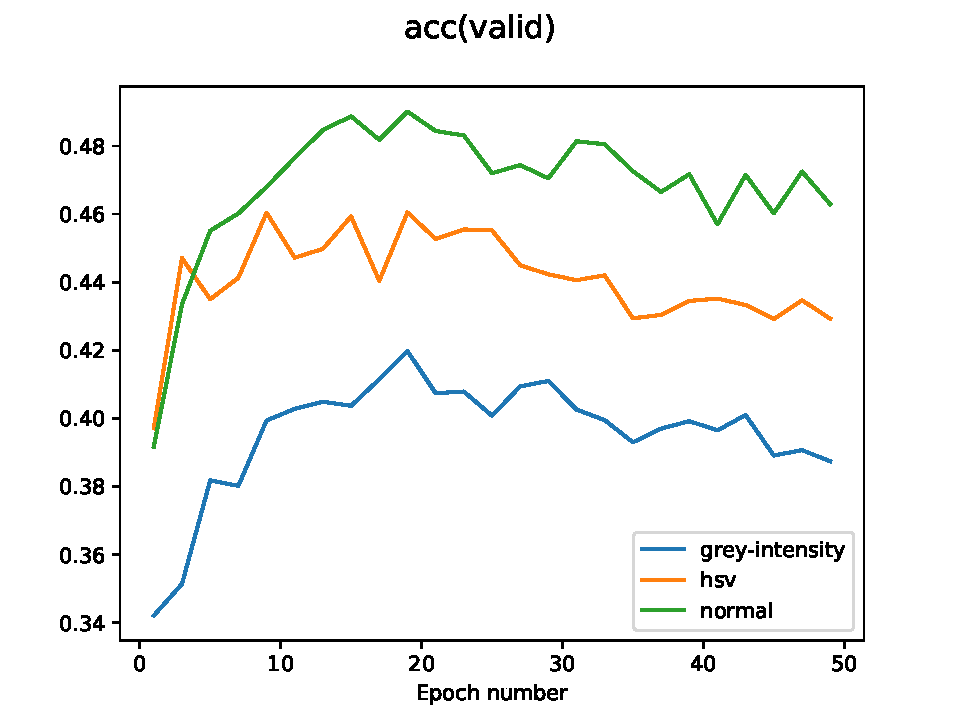
\includegraphics[width=0.5\textwidth]{colour_comp.pdf}

  \caption{Effect of pre-porcessing the CIFAR dataset by transforming into different colour spaces on classification performance. Trained using AdamOptimizer with 3 layers of 200 units each.}
  \label{fig:colour}
\end{figure}

\begin{table}[H]
\centering
\begin{tabular}[h]{| c | c |}
\hline
RGB - original &   243083ms\\
\hline
HSV &   270901ms\\
\hline
greyscale &   138732ms \\
\hline
\end{tabular} 
\caption{Effect of pre-porcessing the CIFAR dataset by transforming into different colour spaces on training time.}
\label{tab:colour}
\end{table}

Greyscale pre-processing shows a significant time saving, however a larger decrease in classification performance than initially expected. For this reason the greyscale dataset will be used to find an appropriate architecture which will be then later trained on the original RGB dataset.

\subsection*{Architectures}

Different model architectures were explored in terms of number of layers and number of hidden units. The exploration was initially done on the greyscale pre-processed dataset after showing that the explored architectures respond similarly to greyscale and RGB input data. A greater number of architectures were explored by leveraging the time saving of having a smaller input dimension of the greyscale datasest. The found best performing greyscale based architectures were compared to the RGB space ones to ensure this correlation was not broken and that an optimal architecture would be found for the RGB space. The explored experiment results are displayed on Figure \ref{fig:arch}, showing that too wide or deep networks are too complex for our dataset as they decrease the classification performance.

\begin{figure*}[ht!]
    \centering
    \begin{subfigure}[t]{0.475\textwidth}
        \centering
        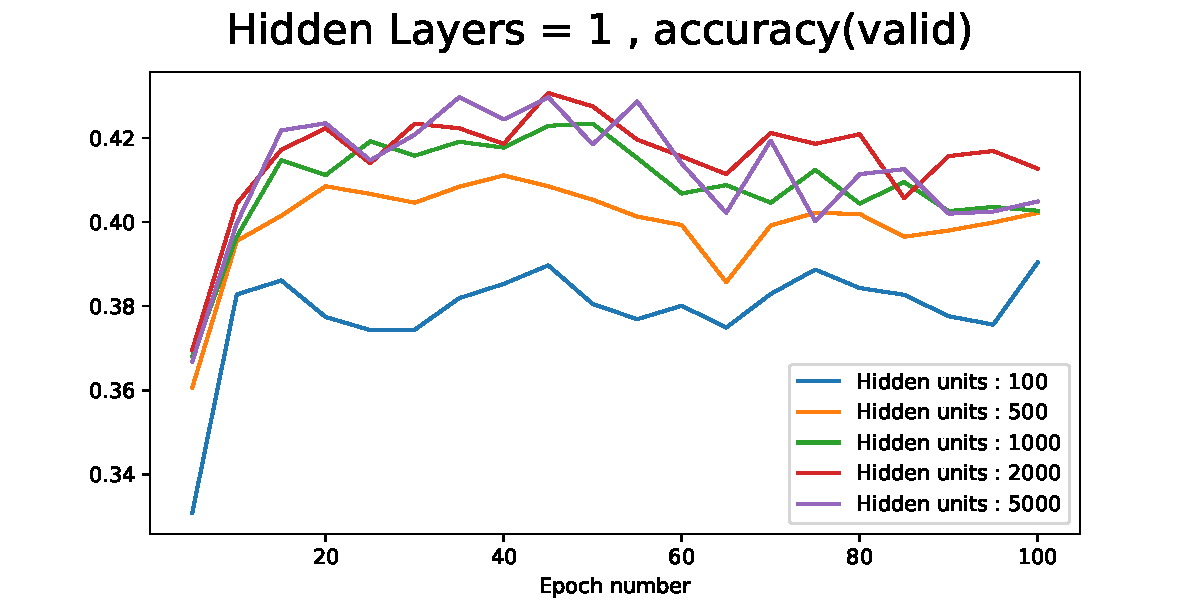
\includegraphics[width=1.0\linewidth]{hidden_units_layers_2_accuracy(valid).pdf}
    \end{subfigure}%
    ~ 
    \begin{subfigure}[t]{0.475\textwidth}
        \centering
        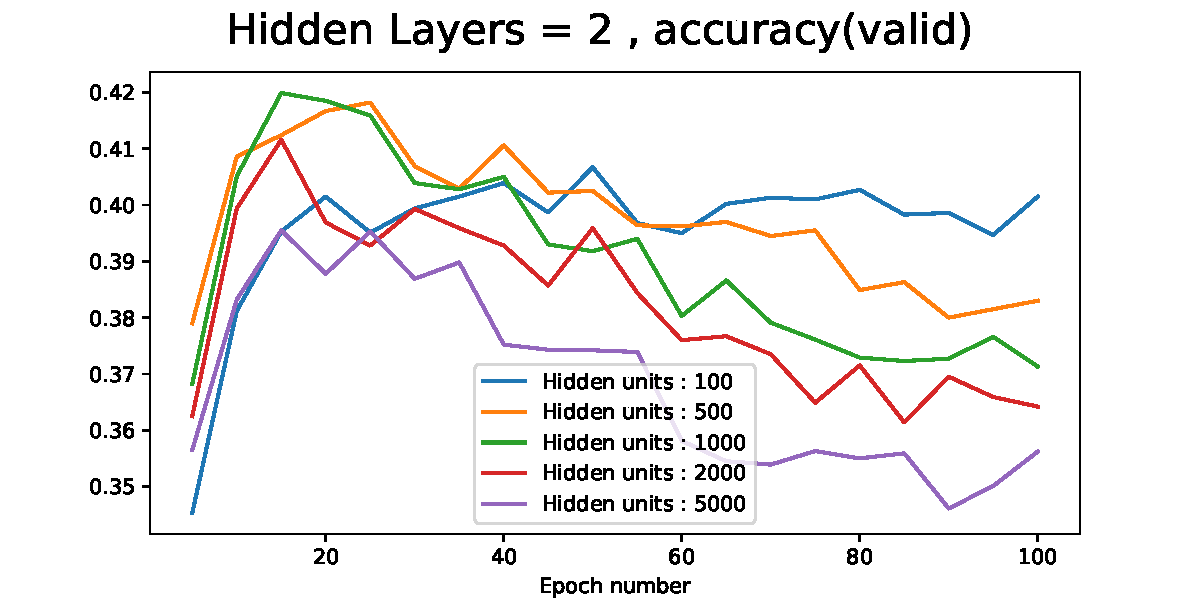
\includegraphics[width=1.0\linewidth]{hidden_units_layers_3_accuracy(valid).pdf}
    \end{subfigure}
    ~
    \begin{subfigure}[t]{0.475\textwidth}
        \centering
        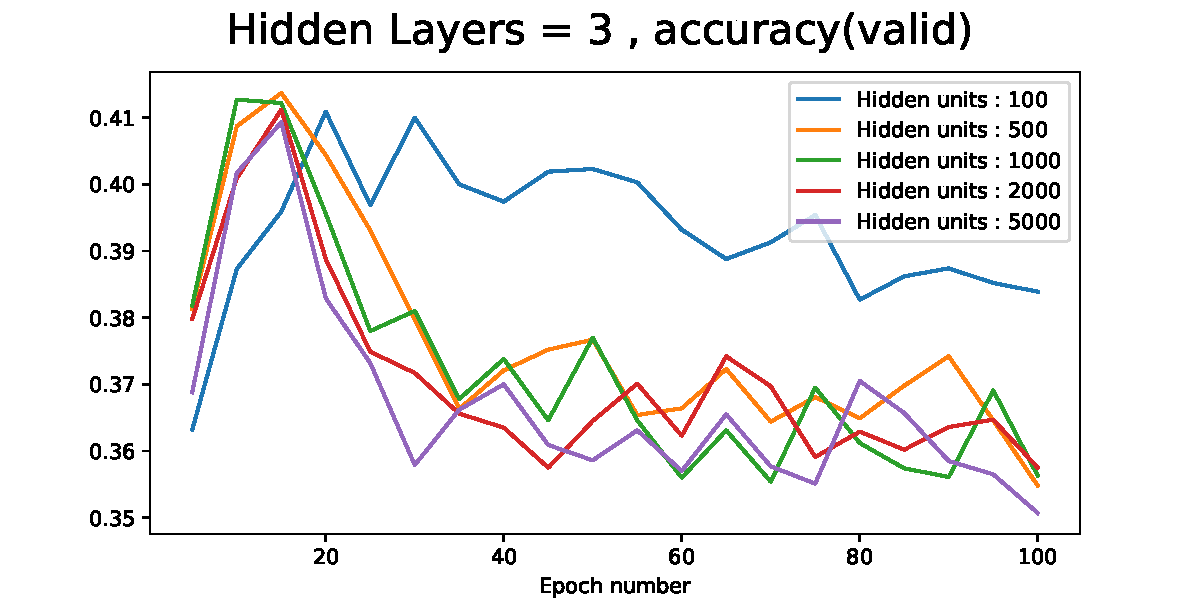
\includegraphics[width=1.0\linewidth]{hidden_units_layers_4_accuracy(valid).pdf}
    \end{subfigure}
    ~
    \begin{subfigure}[t]{0.475\textwidth}
        \centering
        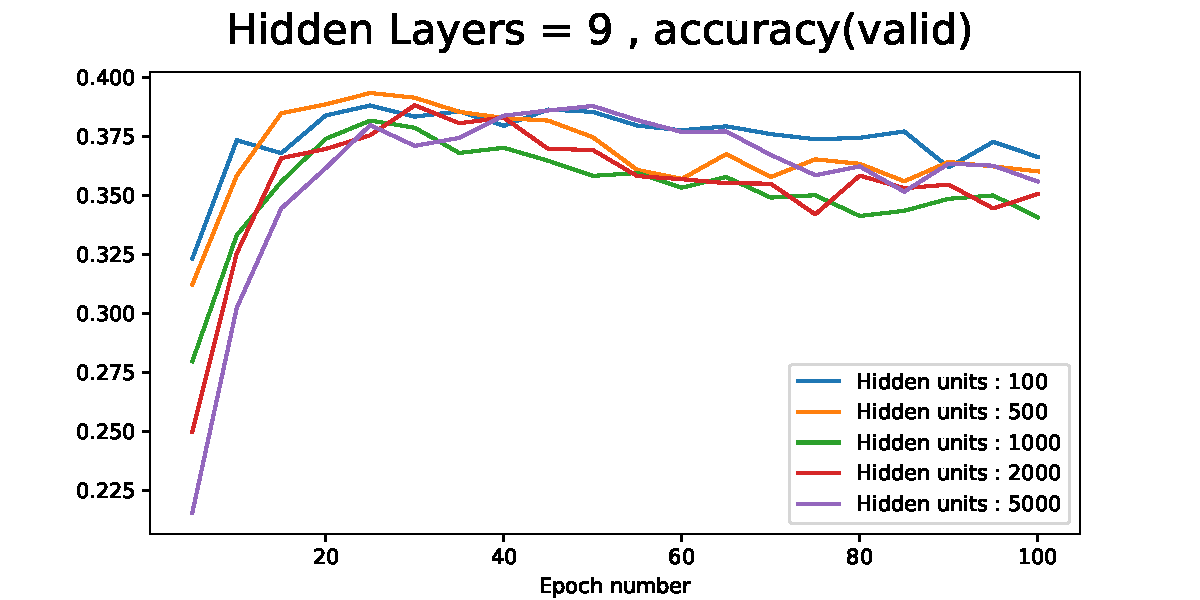
\includegraphics[width=1.0\linewidth]{hidden_units_layers_10_accuracy(valid).pdf}
    \end{subfigure}
    \caption{Classification accuracy comparison on architectures with different numbers of layers and hidden units. }
    \label{fig:arch}
\end{figure*}

The original RGB dataset was then tested on the well performing networks. The results pointing towards several similar good candidates 2 layer architecture of 500 units, or 3 architecture of 200. As these produce good results whilst keeping the number of hidden unit to a minimum. A number of 3 layer architectures were experimented with to confirm this on the RGB dataset as can be seen on Figure \ref{fig:arch2}.

\begin{figure}[H]
\centering
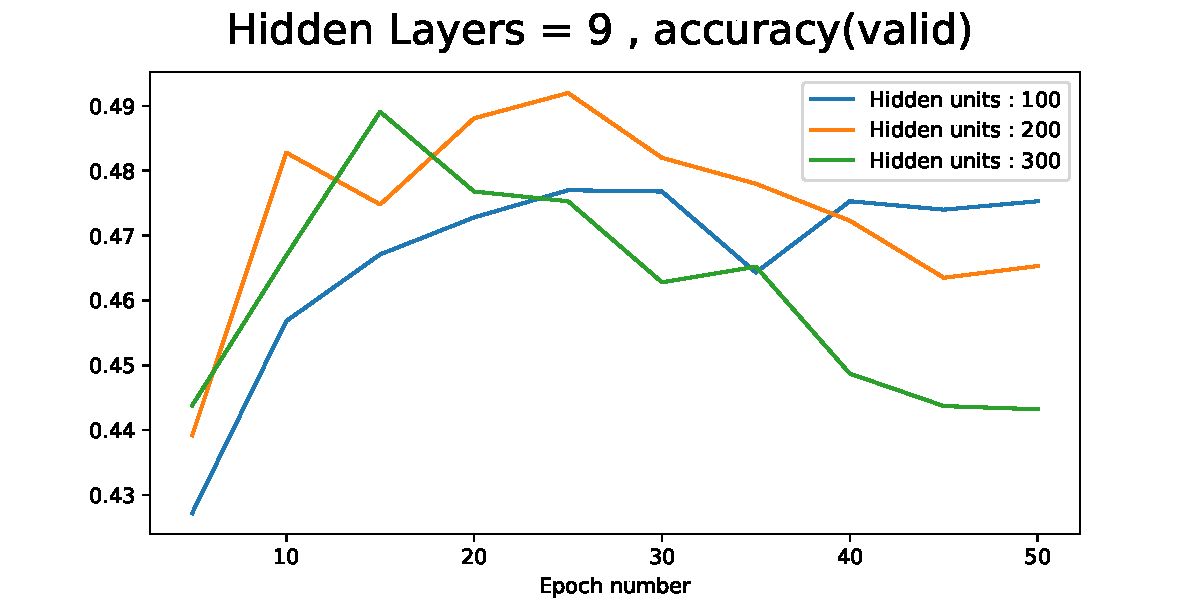
\includegraphics[width=0.5\textwidth]{hidden_units_layers_4_accuracy(valid)_orig.pdf}

  \caption{Classification accuracy for RGB dataset on a 3 layer architecture.}
  \label{fig:arch2}
\end{figure}

Based on the experiments the chosen structure was 3 layers of 200 hidden units each for the original dataset allowing for quite high training speed due to a small overall number of hidden units.

\subsection*{Learning rate update rules}

A number of different learning rate update rules or optimizers were explored to see their effect on this dataset. The tested optimizers were : Gradient Descent, Momentum, Adam\cite{Adam}, AdaGrad\cite{Ada}, AdaDelta\cite{AdaD}. The classification accuracy using each of these with their default parameters can be seen on Figure \ref{fig:opt}. The results showing signifcant improvements over Adam using  gradient descent or AdaGrad optimizers. For all further experiments AdaGrad was chosed due to it's performance and robustness with a learning rate of 0.01. These expriments have shown that the right choice of a learning rate update rule can have a significant effect on the model's accuracy.

\begin{figure}[H]
\centering
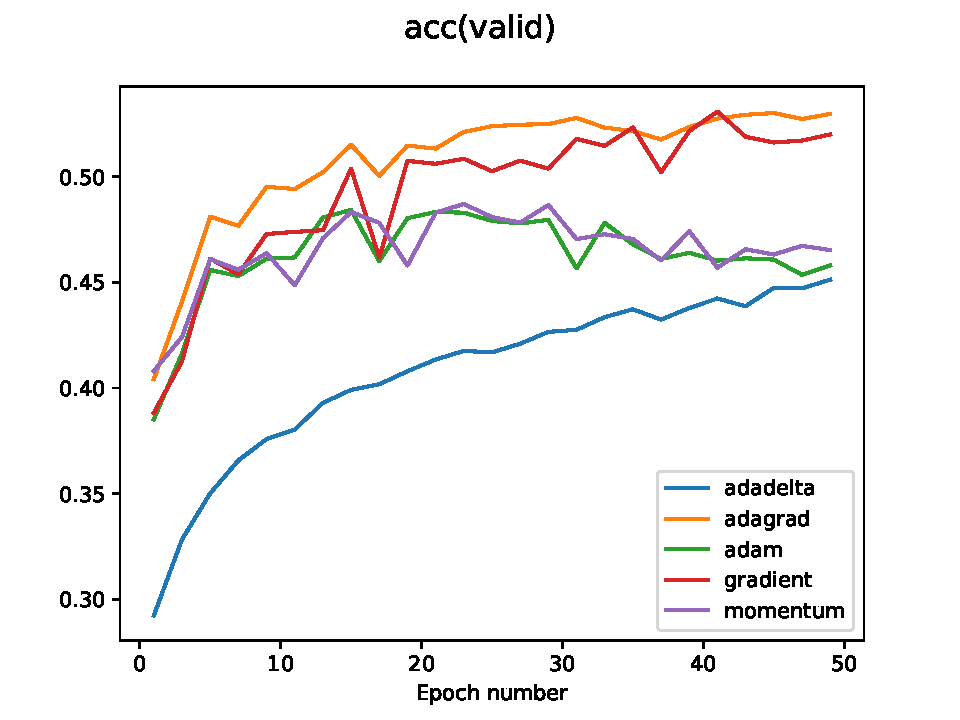
\includegraphics[width=0.7\textwidth]{optimization.pdf}

  \caption{Classification accuracy for different Learning rate update rules trained on a 3 layer network of 200 hidden units per layer.}
  \label{fig:opt}
\end{figure}

\subsection*{Data Augmentation}

Data Augmentation can be seen as a form of regularization and fights sparse training sets. Both of these features are useful here, regularization will prevent our model for CIFAR-10 over-fitting to the training set, while creating new data will be especially useful for the sparse CIFAR-100. In the previous coursework ,various common data augmentations were explored with regards to the MNIST dataset : rotation, shifting, random noise. Rotation for example performed exceptionally well due to people often writing digits under an angle. While random noise had little effect since the dataset has already been cleaned. These examples suggest that when thinking about data augmentations one needs to think what makes sense with regards to the dataset. In the case of CIFAR, rotations would not be expected to help as they would correspond to the picture just being taken under a slight angle. However random noise\cite{grey2} (salt and pepper) could be of use here as the dataset has not been cleaned. Papers\cite{Flip} refer to horizontal reflection as to a helpful data augmentation, which is very logical if one images for example a photo of a horse, flipping this image would transform it as if it were standing the opposite way which is a common occurrence on images. Figure \ref{fig:aug} shows a couple of data augmentation functions with their best performing parameters all applied randomly to 25\% of each batch. The specific parameters for contrast being multiplying by a factor of 0.1 and for noise adding/subtracting a small factor less than 0.1. 


\begin{figure}[H]
\centering
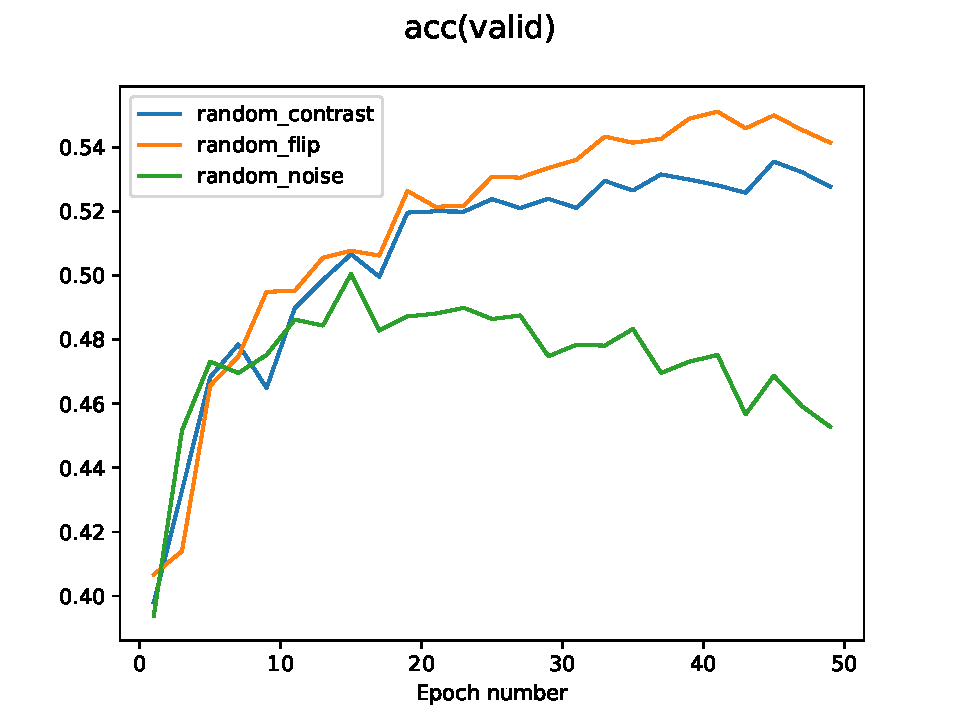
\includegraphics[width=0.7\textwidth]{augmentation.pdf}

  \caption{Classification accuracy when applying different functions for data augmentation.}
  \label{fig:aug}
\end{figure}

Other explored augmentations were random brightness and a mix of well performing augmentation, randomly applying a flip or change of contrast. However, neither of these produced a better result than just flipping on it's own which is what was added to the final model.

\subsection*{Regularization}

The topic of regularization was also explored. Data augmentation can be seen as a form of regularization on it's own. L2 (beta = 0.001) and dropout (keep prob=0.8) were introduced by themselves and in unison to see whether they can prevent over-fitting and increase the classification accuracy. Figure \ref{fig:reg} compares the model so far and the model with applied regularization.

\begin{figure*}[ht!]
    \centering
    \begin{subfigure}[t]{0.475\textwidth}
        \centering
        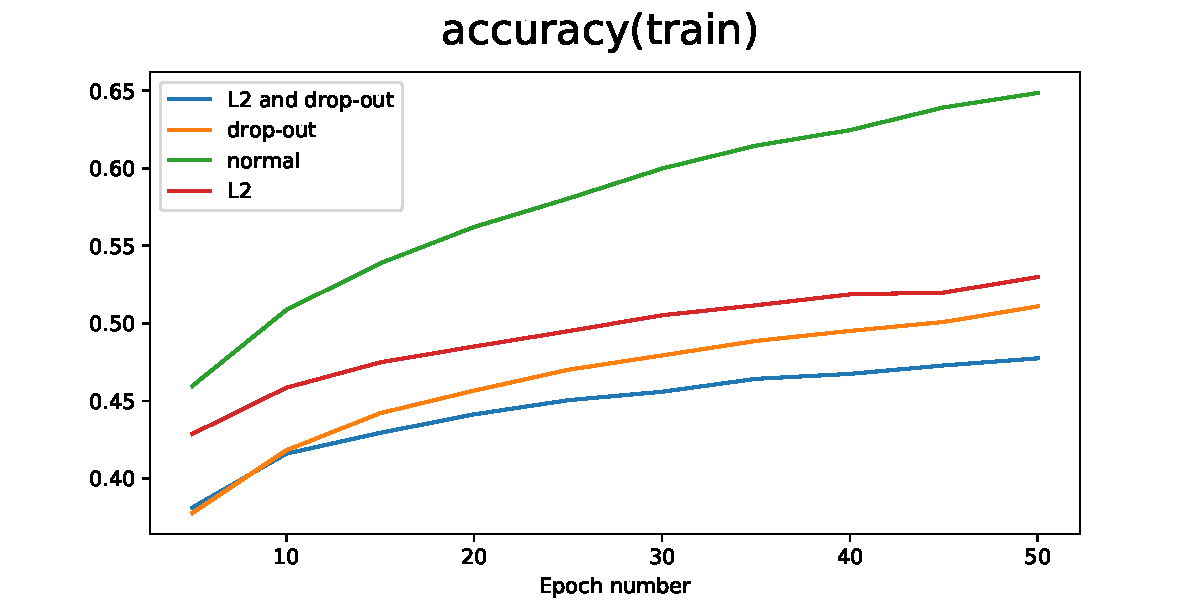
\includegraphics[width=1.0\linewidth]{hidden_units_layers_4_flip_reg_accuracy(train).pdf}
    \end{subfigure}%
    ~ 
    \begin{subfigure}[t]{0.475\textwidth}
        \centering
        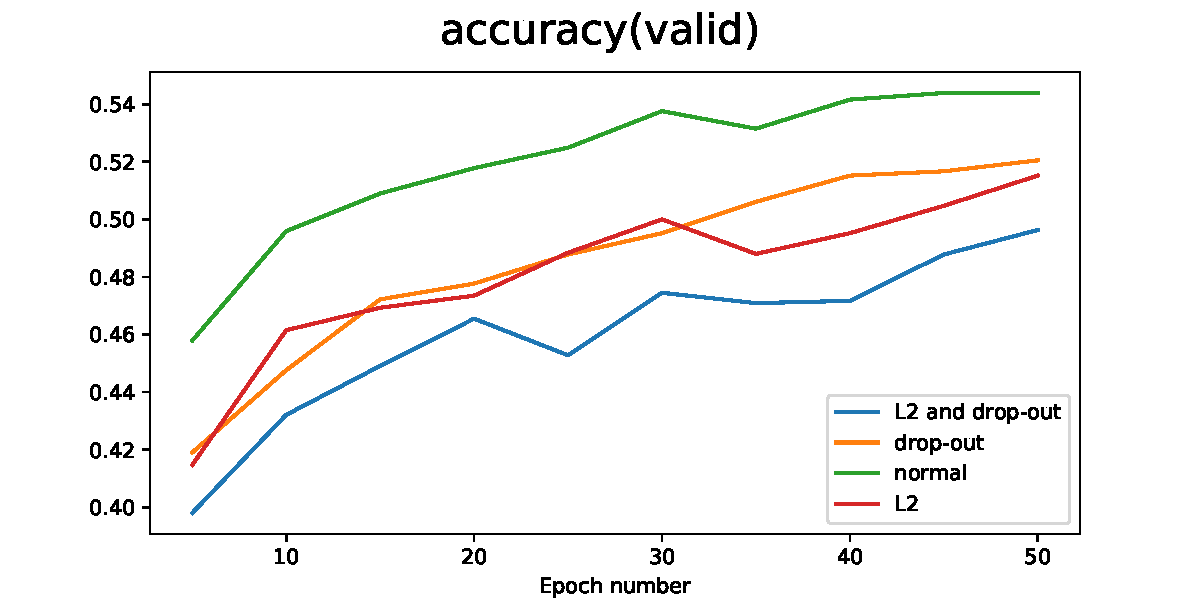
\includegraphics[width=1.0\linewidth]{hidden_units_layers_4_flip_reg_accuracy(valid).pdf}
    \end{subfigure}
   \caption{Effects of L2 and dropout regularization }
    \label{fig:reg}
\end{figure*}

The results showed decrease in performance when using both L2 or dropout alone and together in contrast to a network without these. These methods made the model too rigid, it was not over-fitting but it was also unable to properly capture the data. Therefor, regularization was not introduced to our final model.

\subsection*{Implementation}

The network in use has been built using Tensorflow, this section touches on what has been added compared to the vanilla code provided. The features mentioned will go in line with the order of sections above. Data pre-processing consisted of a script which read the original npz file to transform in to a different colour space. The dataset has been pre-processed as doing this operation on-the-fly proved to be too slow.
The model consisted of a number of fully connected layers as were provided in the vanilla code. Tensorflow's train library was leveraged for all optimizers used, needing to change only one line in order to switch to a new learning rate schedule. Similarly for regularization, Tensorflow's nn library was used for the L2 and dropout functions.


\subsection*{Discussion}



This section will discuss the results from each of the sections above. All of the models were trained on the CIFAR-10 dataset as this was already a complex enough task and CIFAR-100 would bring a new set of challenges that could not be explored until a solid enough model for CIFAR-10 was created. The largest problem being CIFAR-100's sparsity of data. However a lot of conclusions from CIFAR-10 are transferable, the grayscale pre-pocessing and most importantly data-augmentation. However CIFAR-100 would likely need a different architecture, for this reason the dataset will be explored in the next coursework using the results from CIFAR-10.
\\


The pre-porcessed datasets were divided into two cathegories : coloured (HSV,RGB) and greyscale(various algorithms). As expected the coloured datasets performed better as they had 3 times larger dimension than the greyscale. The smaller dimension allowed to train on the greyscale dataset faster. For this reason the greyscale dataset was used to find an appropriate architecture for the RGB colour space later on since it was shown that the performance of both correlated to the same architectures. For futher work some experiments could be devised to try to lessen the difference in accuracy between the RGB and greyscale.
\\


When looking for an appropriate architecture two things were kept in mind : the performance and the speed of training which was dependent on the number of total hidden units. Intuitively too wide or too deep networks did not perform exceptionally well as they were trying to learn too complicated features. Further interesting experiments would regard not having a constant number of units per layer, rather a pyramid shape to the softmax layer.
\\


Data Augmentation had a great positive impact on the overall performance. It has also showed the importance of choosing logical augmentation functions for the dataset as demonstrated by the horizontal flipping example.
\\

The introductions of regularization did not achieve the desired results as it worsened the overall accuracy. The possible cause was that it made the model too rigid to a point where it was not able to learn enough about the dataset even when the regression parameters were rather small. This could be different if the architecture were more complex as 3 layers of 200 units is rather small. Experimenting with effects of regularization on larger architectures could be interesting.




\subsection*{Conclusion}

Overall the model found was a success as it improved the performance over the vanilla neural network by over 13\%. The parameters of the network could be further optimized to achieve even a higher performance by running a grid search using tools like Spearmint on multiple parameters including number of hidden units, data augmentation parameters and learning rates. However even better results are expected to be achieved by introducing convolution in the next coursework.



\begin{thebibliography}{1}
\bibitem{grey1} Shawn McCann, Jim Reesman {\em Object Detection using Convolutional Neural Networks} 
\bibitem{grey2} Dan Ciresan, Ueli Meier, Jurgen Schmidhuber {\em Multi-column Deep Neural Networks for Image Classification}, 2012
\bibitem{grey3} Tanner Helland {\em Seven greyscale conversion algorithms (with pseudocode and VB6 source code)}, http://www.tannerhelland.com/3643/greyscale-image-algorithm-vb6/
\bibitem{Ada} Duchi et al, http://jmlr.org/papers/v12/duchi11a.html
\bibitem{Adam} Kingma, Ba, https://arxiv.org/abs/1412.6980
\bibitem{AdaD} Matthew D. Zeiler {\em ADADELTA An Adaptive Learning Rate Method}
\bibitem{Flip} Alex Krizhevsky, Ilya Sutskever, Geoffrey E. Hinton {\em ImageNet Classification with Deep Convolutional Neural Networks}


\end{thebibliography}

\end{document}
